%!TEX program = xelatex
\documentclass[dvipsnames, svgnames,a4paper,11pt]{article}
% ----------------------------------------------------
%   中山大学物理与天文学院本科实验报告模板
%   作者:Huanyu Shi,2019级
%   知乎:https://www.zhihu.com/people/za-ran-zhu-fu-liu-xing
%   Github:https://github.com/Huanyu-Shi/SYSU-SPA-Labreport-Template
%   Last update : 2023.4.10
% ----------------------------------------------------

% ----------------------------------------------------- 
%	加边框的命令
%	参考:https://tex.stackexchange.com/questions/531559/how-to-add-the-page-border-for-first-two-pages-in-latex
\usepackage{tikz}
\usetikzlibrary{calc}
\usepackage{eso-pic}
\AddToShipoutPictureBG{%
\begin{tikzpicture}[overlay,remember picture]
\draw[line width=0.6pt] % 边框粗细
    ($ (current page.north west) + (0.6cm,-0.6cm) $)
    rectangle
    ($ (current page.south east) + (-0.6cm,0.6cm) $); % 边框位置
\end{tikzpicture}}


\usepackage{xcolor}
\definecolor{c1}{HTML}{2752C9} % 目录颜色
\definecolor{c2}{RGB}{190,20,83} % 引用颜色

\usepackage{ctex}
\usepackage[top=28mm,bottom=28mm,left=15mm,right=15mm]{geometry} % 调整边距
\usepackage{hyperref} 
\hypersetup{
	colorlinks,
	linktoc = section, % 超链接位置,选项有section, page, all
	linkcolor = c1, % linkcolor 目录颜色
	citecolor = c1  % citecolor 引用颜色
}
\usepackage{amsmath,enumerate,multirow,float}
\usepackage{tabularx}
\usepackage{tabu}
\usepackage{subfig}
\usepackage{fancyhdr}
\usepackage{graphicx}
\usepackage{wrapfig}  
\usepackage{physics}
\usepackage{appendix}
\usepackage{amsfonts}
\usepackage{annotate-equations} % 公式标注
\usepackage{pgfplots}


% ---------------------------------------------------------------------
%	定义了两类colorbox
\usepackage{tcolorbox}
\tcbuselibrary{skins,breakable}
\newtcolorbox{tbox}[2][]{
    colframe=black!70!,
    breakable,
    enhanced,
	boxrule =0.5pt,
    title = {#2},
    fonttitle = \large\bfseries,
	drop fuzzy shadow,
    #1
}
\newtcolorbox[auto counter,number within=section]{question}[1][]{
  top=2pt,bottom=2pt,arc=1mm,
  boxrule=0.5pt,
%   frame hidden,
  breakable,
  enhanced, %跨页后不会显示下边框
  coltitle=c1!80!gray,
  colframe=c1,
  colback=c1!3!white,
  drop fuzzy shadow,
  title={思考题~\thetcbcounter:\quad},
  fonttitle=\bfseries,
  attach title to upper,
  #1
}

% ---------------------------------------------------------------------
%	利用cleveref改变引用格式,\cref是引用命令
\usepackage{cleveref}
\crefformat{figure}{#2{\textcolor{c2}{图 #1}}#3} % 图片的引用格式
\crefformat{equation}{#2{(\textcolor{c2}{#1})}#3} % 公式的引用格式
\crefformat{table}{#2{\textcolor{c2}{表 #1}}#3} % 表格的引用格式


% ---------------------------------------------------------------------
%	页眉页脚设置
\fancypagestyle{plain}{\pagestyle{fancy}}
\pagestyle{fancy}
\lhead{\kaishu 中山大学物理与天文学院物理实验\uppercase\expandafter{\romannumeral3}} % 左边页眉,学院 + 课程
\rhead{\kaishu Template 实验报告模板} % 右边页眉,实验报告标题
\cfoot{\thepage} % 页脚,中间添加页码
\setlength{\headheight}{13.6pt}

% ---------------------------------------------------------------------
%	对目录、章节标题的设置
\renewcommand{\contentsname}{\centerline{\huge 目录}}
\usepackage{titlesec}
\usepackage{titletoc}
% \titleformat{章节}[形状]{格式}{标题序号}{序号与标题间距}{标题前命令}[标题后命令]
\titleformat{\section}{\centering\LARGE}{}{1em}{}
\newcommand{\nsection}[3]{%
    \section{#1 #2 \hspace{11pt} \textbf{#3}}%
}

% ---------------------------------------------------------------------
%   listing代码环境设置
\usepackage{listings}
\lstloadlanguages{python}
\lstdefinestyle{pythonstyle}{
backgroundcolor=\color{gray!5},
language=python,
frameround=tftt,
frame=shadowbox, 
keepspaces=true,
breaklines,
columns=spaceflexible,                   
basicstyle=\ttfamily\small, % 基本文本设置,字体为teletype,大小为scriptsize
keywordstyle=[1]\color{c1}\bfseries, 
keywordstyle=[2]\color{Red!70!black},   
stringstyle=\color{Purple},       
showstringspaces=false,
commentstyle=\ttfamily\scriptsize\color{green!40!black},%注释文本设置,字体为sf,大小为smaller
tabsize=2,
morekeywords={as},
morekeywords=[2]{np, plt, sp},
numbers=left, % 代码行数
numberstyle=\it\tiny\color{gray}, % 代码行数的数字字体设置
stepnumber=1,
rulesepcolor=\color{gray!30!white}
}


% ---------------------------------------------------------------------
%	将表格封装起来
\newcommand{\scoresTable}[8]{
    \begin{table}
        \renewcommand\arraystretch{1.7}
        \begin{tabularx}{\textwidth}{
                |X|X|X|X
                |X|X|X|X|}
            \hline
            \multicolumn{2}{|c|}{预习报告} & \multicolumn{2}{|c|}{实验记录} & \multicolumn{2}{|c|}{分析讨论} & \multicolumn{2}{|c|}{总成绩} \\
            \hline
            \centering#1&\centering#2 &\centering#3 &\centering#4 &\centering#5 &\centering#6 &\centering#7 &{\centering#8} \\
            \hline
        \end{tabularx}
    \end{table}
}
\newcommand{\infoTable}[6]{
    \begin{table}
        \renewcommand\arraystretch{1.7}
        \begin{tabularx}{\textwidth}{|X|X|X|X|}
        \hline
        专业:& #1 &年级:& #2\\
        \hline
        姓名:& #3   & 学号:&#4\\
        \hline
        实验时间:&#5 & 教师签名:&#6 \\
        \hline
        \end{tabularx}
    \end{table}
}

% ---------------------------------------------------------------------
%	其他设置
\def\degree{${}^{\circ}$} % 角度
\graphicspath{{./images/}} % 插入图片的相对路径
\allowdisplaybreaks[4]  %允许公式跨页

\usetikzlibrary{patterns,decorations.markings,arrows.meta,bending} % 导入模板的相关设置
\usepackage{lipsum}


%---------------------------------------------------------------------
%	正文
%---------------------------------------------------------------------

\begin{document}


\begin{table}
	\renewcommand\arraystretch{1.7}
	\begin{tabularx}{\textwidth}{
		|X|X|X|X
		|X|X|X|X|}
	\hline
	\multicolumn{2}{|c|}{预习报告}&\multicolumn{2}{|c|}{实验记录}&\multicolumn{2}{|c|}{分析讨论}&\multicolumn{2}{|c|}{总成绩}\\
	\hline
	& & & & & & & \\
	\hline
	\end{tabularx}
\end{table}


\begin{table}
	\renewcommand\arraystretch{1.7}
	\begin{tabularx}{\textwidth}{|X|X|X|X|}
	\hline
	专业:& 物理学 &年级:& 2019级\\
	\hline
	姓名:&   & 学号:&\\
	\hline
	实验时间:& & 教师签名:& \\
	\hline
	\end{tabularx}
\end{table}

\begin{center}
	\LARGE Template \quad 实验报告模板
\end{center}

\textbf{【实验报告注意事项】}
\begin{enumerate}
	\item 实验报告由三部分组成:
	\begin{enumerate}
		\item 预习报告:(提前一周)认真研读\underline{\textbf{实验讲义}},弄清实验原理;实验所需的仪器设备、用具及其使用(强烈建议到实验室预习),完成课前预习思考题;了解实验需要测量的物理量,并根据要求提前准备实验记录表格(第一循环实验已由教师提供模板,可以打印)。预习成绩低于10分(共20分)者不能做实验。
	    \item 实验记录:认真、客观记录实验条件、实验过程中的现象以及数据。实验记录请用珠笔或者钢笔书写并签名(\textcolor{red}{\textbf{用铅笔记录的被认为无效}})。\textcolor{red}{\textbf{保持原始记录,包括写错删除部分,如因误记需要修改记录,必须按规范修改。}}(不得输入电脑打印,但可扫描手记后打印扫描件);离开前请实验教师检查记录并签名。
	    \item 分析讨论:处理实验原始数据(学习仪器使用类型的实验除外),对数据的可靠性和合理性进行分析;按规范呈现数据和结果(图、表),包括数据、图表按顺序编号及其引用;分析物理现象(含回答实验思考题,写出问题思考过程,必要时按规范引用数据);最后得出结论。
	\end{enumerate}
	\textbf{实验报告就是将预习报告、实验记录、和数据处理与分析合起来,加上本页封面。}
	\item 每次完成实验后的一周内交\textbf{实验报告}(特殊情况不能超过两周)。
	\item 除实验记录外,实验报告其他部分建议双面打印。
\end{enumerate}


\clearpage
\tableofcontents
\clearpage

\setcounter{section}{0}
\section{Template 光电效应实验 \quad\heiti 预习报告}
	
\subsection{实验目的}
\begin{enumerate}
	\item 了解光电效应的规律,加深对光的量子性的理解;
	\item 测量不同光频率下的截止电压,计算普朗克常量$h$,测量光电管的伏安特性。
\end{enumerate}

\subsection{仪器用具}
\begin{table}[htbp]
	\centering
	\renewcommand\arraystretch{1.6}
	% \setlength{\tabcolsep}{10mm}
	\begin{tabular}{p{0.05\textwidth}|p{0.20\textwidth}|p{0.05\textwidth}|p{0.5\textwidth}}
	\hline
	编号& 仪器用具名称 & 数量 &  主要参数(型号,测量范围,测量精度等) \\
	\hline
	1&高压汞灯 &1 & BEM-5005, 50W/220 VAC,谱线:365nm, 405nm, 436nm, 546nm, 577nm\\

	2&光电管 &1 & BEM-5006, 光谱响应范围:300-700 nm,滤光片(中心波长分别为365nm, 405nm, 436nm, 546nm, 577nm),
	光阑(直径分别为2mm, 4mm, 8mm)、遮光盖、线缆等 \\
	
	3&微电流放大器 & 1 &BEM-5004 \\
	
	4&可调直流电源&1 & GPP-4323, 4通道, 32V/3A$\times$2 (CH1/CH2), 5V/1A (CH3), 15V/1A (CH4)\\
	\hline
\end{tabular}
\end{table}

\subsection{原理概述}
\begin{wrapfigure}{l}{0cm} % l表示靠文字内容的左侧,0cm表示环境横向长度
	\centering
	
\includegraphics[width=0.3\textwidth]{example.png}
	\caption{环绕图片示例}
\end{wrapfigure}
\textcolor{red}{参考文献示例},参考\cite{test1,test2}。

光电效应(英语:Photoelectric Effect)是指光束照射物体时会使其发射出电子的物理效应。发射出来的电子称为“光电子”。

光束里的光子所拥有的能量与光的频率成正比。假若金属里的电子吸收了一个光子的能量,而这能量大于或等于某个与金属相关的能量阈值(称为这种金属的逸出功),
则此电子因为拥有了足够的能量,会从金属中逃逸出来,成为光电子;若能量不足,则电子会释出能量,能量重新成为光子离开,电子能量恢复到吸收之前,
无法逃逸离开金属。增加光束的辐照度(光束的强度)会增加光束里光子的密度,在同一段时间内激发更多的电子,但不会
使得每一个受激发的电子因吸收更多的光子而获得更多的能量。换言之,光电子的能量与辐照度无关,只与光子的能量、频率有关。

被光束照射到的电子会吸收光子的能量,但是其中机制遵照的是一种非全有即全无的准则,光子所有能量都必须被吸收,用来克服逸出功,
否则这能量会被释出。假若电子所吸收的能量能够克服逸出功,并且还有剩馀能量,则这剩余能量会成为电子在被发射后的动能。

逸出功$W_0$是从金属表面发射出一个光电子所需要的最小能量。如果转换到频率的角度来看,光子的频率必须大于金属特征的极限频率,
才能给予电子足够的能量克服逸出功。逸出功与极限频率$\nu_0$之间的关系为
\begin{equation}
	W_0 = h\nu_0
\end{equation}
其中,$h$是普朗克常数,$h\nu_0$是光频率为$\nu_0$的光子的能量。

克服逸出功之后,光电子的最大动能$E_{\max}$为
\begin{equation}
	E_{\max} = h\nu - W_0 = h(\nu-\nu_0)
\end{equation}
其中,$h\nu$是光频率为$\nu$的光子所带有并且被电子吸收的能量。

实际物理要求动能必须是正值,因此,光频率必须大于或等于极限频率,光电效应才能发生。
\begin{figure}[htbp]
	\centering
	\subfloat[]{
		
\includegraphics[width=0.3\textwidth]{example.png}
	}
	\subfloat[]{
		
\includegraphics[width=0.3\textwidth]{example.png}
	}
	\subfloat[]{
		
\includegraphics[width=0.3\textwidth]{example.png}
	}

	\subfloat[]{
		
\includegraphics[width=0.3\textwidth]{example.png}
	}
	\subfloat[]{
		
\includegraphics[width=0.3\textwidth]{example.png}
	}
	\subfloat[]{
		
\includegraphics[width=0.3\textwidth]{example.png}
	}
	\caption{多行多列图片示例}
\end{figure}

\subsection{实验安全注意事项}
\begin{enumerate}
	\item 实验过程中,禁止汞灯光线直接照射光电管,也不宜长时间连续照射加有光阑和滤光片的光电管。\textcolor{red}{\textbf{仪器暂不使用时,均须将汞灯和光电管盒用遮光盖盖上。}}
	\item \textcolor{red}{\textbf{ 实验过程中,禁止用眼睛直视汞灯的出射光。}}
	\item 实验完成后,需将光电管盒的遮光盖盖上,以保护光电管。
	\item 汞灯和电源在测量前需要预热20分钟。汞灯光源功率为50W,温度较高\textcolor{red}{\textbf{须防止烫伤。}}
	\item 切换滤光片时直接旋转滤光器,切换光阑时需要略微向外拔出一点,旋转到需要的光阑
	尺寸后光阑会自动复位。
	\item 注意:切换微电流放大器档位后,需要调零,否则会影响实验精度。	
\end{enumerate}

\subsection{实验前思考题}
\begin{question}
	这是一道实验前思考题,\lipsum[10]
\end{question}
你可以在这里写答案

\begin{question}
	这是另一道实验前思考题,\lipsum[11]
	\tcblower
	你也可以在这里写答案,\lipsum[12]
\end{question}

\clearpage
\begin{table}
	\renewcommand\arraystretch{1.7}
	\centering
	\begin{tabularx}{\textwidth}{|X|X|X|X|}
	\hline
	专业:& 物理学 &年级:& 2019级 \\
	\hline
	姓名: & & 学号:&\\
	\hline
	室温:& & 实验地点: & \\
	\hline
	学生签名:& & 评分: &\\
	\hline
	实验时间:& & 教师签名:&\\
	\hline
	\end{tabularx}
\end{table}

\section{Template 光电效应实验 \quad\heiti 实验记录}
\subsection{实验内容和步骤}
\subsection{实验数据记录}
\subsection{原始数据记录}
\subsection{实验过程中遇到的问题记录}



\clearpage
\begin{table}
	\renewcommand\arraystretch{1.7}
	\begin{tabularx}{\textwidth}{|X|X|X|X|}
	\hline
	专业:& 物理学 &年级:& 2019级\\
	\hline
	姓名: & & 学号:& \\
	\hline
    日期:& & 评分: &\\
	\hline
	\end{tabularx}
\end{table}

\section{Template 光电效应实验 \quad\heiti 分析与讨论}
\subsection{实验数据分析}
\subsection{实验后思考题}
\begin{question}
	这是一道实验后思考题,\lipsum[20]
\end{question}

\clearpage
% ---------------------------------------------------------------------
%   参考文献
%   注:使用参考文献时应按照xelatex->bibtex->xelatex->xelatex顺序进行编译
\phantomsection
\addcontentsline{toc}{section}{参考文献}
\bibliographystyle{unsrt}
\bibliography{myref}

\clearpage
\appendix
\appendixpage
\addappheadtotoc
\subsection{代码记录}
\begin{lstlisting}[style=pythonstyle,caption=代码记录示例]
	import matplotlib.pyplot as plt
	import numpy as np
	
	# Data for plotting
	t = np.arange(0.0, 2.0, 0.01)
	s = 1 + np.sin(2 * np.pi * t)
	
	fig, ax = plt.subplots()
	ax.plot(t, s)
	
	ax.set(xlabel='time (s)', ylabel='voltage (mV)',
		   title='About as simple as it gets, folks')
	ax.grid()
	
	fig.savefig("test.png")
	plt.show()
\end{lstlisting}
\begin{figure}[H]
    \centering
    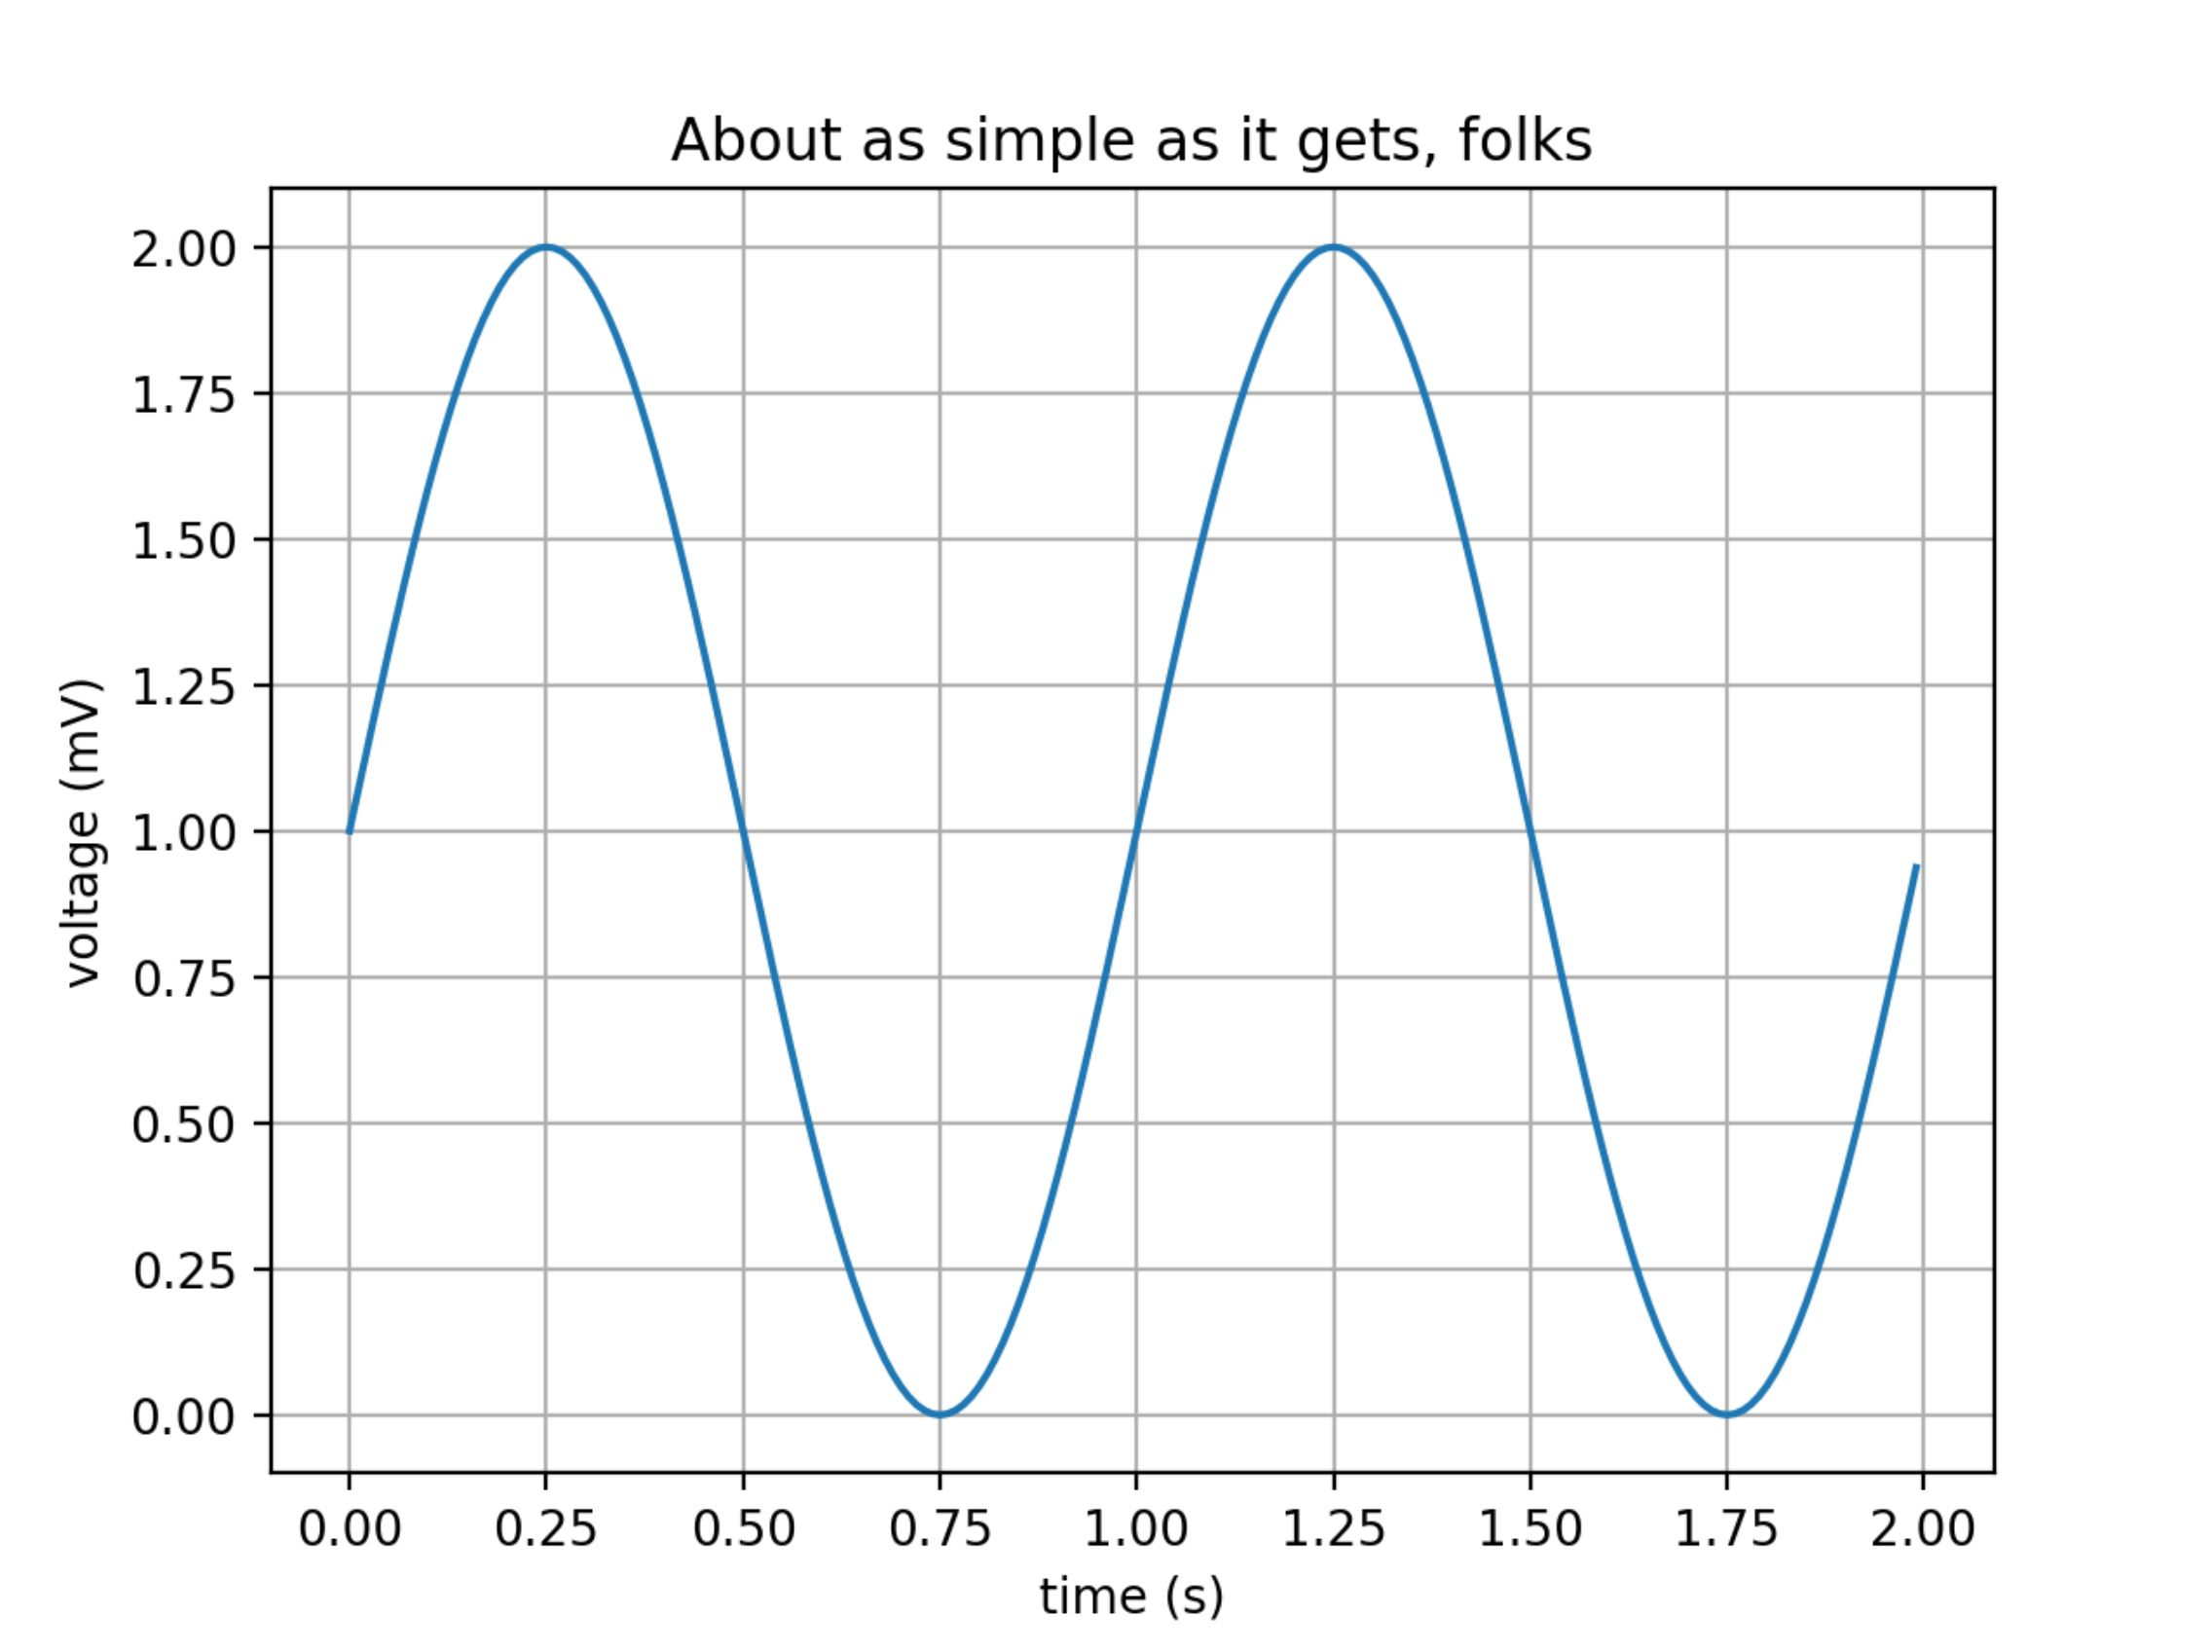
\includegraphics[width = 0.6\textwidth]{example1.png}
    \caption{Test Figure}
\end{figure}

\clearpage
\subsection{常用命令展示}
这部分将展示其他常用命令。

\begin{tbox}{颜色设置}
\begin{itemize}
	\item  \textcolor{Red}{赤}\textcolor{Orange}{橙}\textcolor{Yellow}{黄}\textcolor{Green}{绿}\textcolor{Emerald}{青}\textcolor{Blue}{蓝}\textcolor{Purple}{紫}
	\item  谁持彩练当空舞
\end{itemize}
\end{tbox}

\begin{tbox}{字号设置}
\begin{enumerate}
	\item {\LARGE 江晚正愁余}
	\item {\Large 江晚正愁余}
	\item {\large 江晚正愁余}
	\item {\normalsize 江晚正愁余}
	\item {\small 江晚正愁余}
	\item {\footnotesize 江晚正愁余}
	\item {\scriptsize 江晚正愁余}
\end{enumerate}
\end{tbox}

\begin{tbox}{字体设置(中文)}
\begin{enumerate}
	\item 宋体:{\songti 山有扶苏,隰有荷华}
	\item 仿宋:{\fangsong 山有扶苏,隰有荷华}
	\item 黑体:{\heiti 山有扶苏,隰有荷华}
	\item 楷书:{\kaishu 山有扶苏,隰有荷华}
\end{enumerate}
\end{tbox}

\begin{tbox}{Set font(English)}
\begin{enumerate}
	\item roman:\quad{\rmfamily Hello world!}
	\item sans-serif:\quad{\sffamily Hello world!}
	\item typewriter:\quad{\ttfamily Hello world!}
\end{enumerate}
\end{tbox}

\begin{tbox}{公式}
	无编号公式
    \begin{equation*}
        J(\theta) = \mathbb{E}_{\pi_\theta}[G_t] = \sum_{s\in\mathcal{S}} d^\pi (s)V^\pi(s)=\sum_{s\in\mathcal{S}} d^\pi(s)\sum_{a\in\mathcal{A}}\pi_\theta(a|s)Q^\pi(s,a)
    \end{equation*}
$$ J(\theta) = \mathbb{E}_{\pi_\theta}[G_t] = \sum_{s\in\mathcal{S}} d^\pi (s)V^\pi(s)=\sum_{s\in\mathcal{S}} d^\pi(s)\sum_{a\in\mathcal{A}}\pi_\theta(a|s)Q^\pi(s,a) $$
    有编号公式
    \begin{equation}
        J(\theta) = \mathbb{E}_{\pi_\theta}[G_t] = \sum_{s\in\mathcal{S}} d^\pi (s)V^\pi(s)=\sum_{s\in\mathcal{S}} d^\pi(s)\sum_{a\in\mathcal{A}}\pi_\theta(a|s)Q^\pi(s,a)
    \end{equation}
    \begin{equation}
        J(\theta) = \mathbb{E}_{\pi_\theta}[G_t] = \sum_{s\in\mathcal{S}} d^\pi (s)V^\pi(s)=\sum_{s\in\mathcal{S}} d^\pi(s)\sum_{a\in\mathcal{A}}\pi_\theta(a|s)Q^\pi(s,a)
    \end{equation}
	波尔文积分
    \[
    \begin{cases}
        \vspace{0.2cm}
        \displaystyle{\int_{0}^{\infty} \frac{\sin(x)}{x}\,dx = \frac{\pi}{2}}\\
        \vspace{0.2cm}
        \displaystyle{\int_{0}^{\infty} \frac{\sin(x)}{x} \frac{\sin(x/3)}{x/3}\,dx = \frac{\pi}{2}} \\
        \vspace{0.2cm}\cdot\cdot\cdot\\
        \vspace{0.2cm}
        \displaystyle{\int_{0}^{\infty} \frac{\sin(x)}{x} \frac{\sin(x/3)}{x/3} \cdot\cdot\cdot \frac{\sin(x/13)}{x/13}\,dx = \frac{\pi}{2}}\\
        \displaystyle{\int_{0}^{\infty} \frac{\sin(x)}{x} \frac{\sin(x/3)}{x/3} \cdot\cdot\cdot \frac{\sin(x/15)}{x/15}\,dx = \frac{467807924713440738696537864469}{935615849440640907310521750000}\pi}
    \end{cases}  
    \]
	多行对齐公式
\begin{align*}
    \frac{\partial}{\partial \theta_k}J(\theta) 
        &= \frac{\partial}{\partial \theta_k}\Bigg[\frac{1}{m}\sum_{k=1}^m log(1+e^{-y^{(i)}\theta^Tx^{(i)}})\Bigg] \\
        &= \frac{1}{m}\sum_{k=1}^m \frac{1}{1+e^{-y^{(i)}\theta^Tx^{(i)}}}y^{(i)}x_k^{(i)} \\
        &= -\frac{1}{m}\sum_{k=1}^m h_\theta(-y^{(i)}x^{(i)})y^{(i)}x_k^{(i)}        
\end{align*}
\end{tbox}

\begin{tbox}{引用}
	对公式的引用,如\cref{equ:test}
	\begin{equation}
        J(\theta) = \mathbb{E}_{\pi_\theta}[G_t] = \sum_{s\in\mathcal{S}} d^\pi (s)V^\pi(s)=\sum_{s\in\mathcal{S}} d^\pi(s)\sum_{a\in\mathcal{A}}\pi_\theta(a|s)Q^\pi(s,a)
		\label{equ:test}
    \end{equation}
	对图像的引用,如\cref{fig:test}
	\begin{figure}[H]
		\centering
		
\includegraphics[width=0.3\textwidth]{example.png}
		\caption{测试图片}
		\label{fig:test}
	\end{figure}
	对表格的引用,如\cref{tab:test}
	\begin{table}[H]
		\renewcommand\arraystretch{1.5}
		\caption{一个空表格}
		\begin{tabularx}{\textwidth}{|p{0.15\textwidth}|X|X|X|X|}
		\hline
		 &  &  &  &  \\    
		\hline
		 &  &  & &  \\    
		\hline
		\end{tabularx}
		\label{tab:test}
	\end{table}
\end{tbox}

\begin{tbox}{表格}
	tabular可以自己更改宽度
	\begin{table}[H]
		\renewcommand\arraystretch{1.7}
		\centering
		\caption{一个空表格}
		\begin{tabular}{|p{0.15\textwidth}|p{0.15\textwidth}|p{0.15\textwidth}|p{0.15\textwidth}|}
		\hline
		&   &  &  \\
		\hline
		 &   &  &  \\
		\hline    
		\end{tabular}
	\end{table}
	tabularx可以自适应宽度
	\begin{table}[H]
		\renewcommand\arraystretch{1.7}
		\centering
		\caption{一个空表格}
		\begin{tabularx}{\textwidth}{|p{0.2\textwidth}|X|X|X|X|X|X|}
			\hline
			& &  &  &  &  &  \\
			\hline
			 & &  &  &  &  &  \\
			\hline
		\end{tabularx}
	\end{table}
\end{tbox}
\end{document}
